%
% Categorifying the zx-calculus
% A categoification of zx
% arXiv v2
%

\documentclass[./1--Catfying_zxCalc--Master.tex]{subfiles} % ./mainfilename.tex
%\input{Catfying_zxCalc--Preamble.tex}

%%%%%%%%%%%%%%%%%%
%%%%%%%%%%%%%%%%%%
% 
\begin{document}
%
%%%%%%%%%%%%%%%%%%
%%%%%%%%%%%%%%%%%%

%%%%%%%%%%%%%%%%%%%%%%
%%%%%%%%%%%%%%%%%%%%%%
% ZX CATEGORIFIED
\section{A categorification of $\mathbf{zx}$}
\label{sec:zx categorified}
%%%%%%%%%%%%%%%%%%%%%%
%%%%%%%%%%%%%%%%%%%%%%

Section \ref{sec:OpenGraphsOverSzx} 
describes a translation of
the basic $\mathbf{zx}$-morphisms 
into open graphs over $S_{\text{zx}}$.
These are depicted in 
Figure \ref{fig:ZX 1cells generators}
and are referred to as 
\emph{basic open graphs over $S_{\text{zx}}$}.  
To clarify the double instances of $m$ and $n$ 
written in the spider diagrams, 
those below the diagram 
refer to the cardinalities of the cospan legs, 
and those beside the brackets 
count how many nodes are there
(cf.\ Example \ref{ex:open graph over Szx}).  

\begin{figure}[h]
	\fbox{%
		\begin{minipage}{\textwidth}
			\centering
			%%%%%%%%%%%%%%%%%%%%%%
			\subcaptionbox{Wire}{%
				\centering
				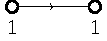
\includegraphics{InclGrphx--1cell--zx_wire}
			}
			\quad \quad \quad \quad
			\subcaptionbox{Hadamard}[2.5cm]{%
				\centering
				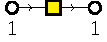
\includegraphics[]{InclGrphx--1cell--zx_hadamard}
			}
			\quad \quad \quad \quad
			\subcaptionbox{Diamond}[2.5cm]{%
				\centering
				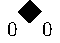
\includegraphics{InclGrphx--1cell--zx_diamond}
			}
			\vspace{1em}
			\linebreak
			%%%%%%%%%%%%%%%%%%%%%
			\subcaptionbox{Green spider}{%
				\centering
				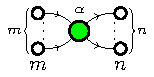
\includegraphics{InclGrphx--1cell--zx_green_spider}
			}
			\quad \quad \quad \quad
			\subcaptionbox{Red spider}{%
				\centering
				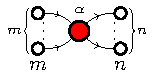
\includegraphics{InclGrphx--1cell--zx_red_spider}
			}
			%%%%%%%%%%%%%%%%%%%%%%
		\end{minipage}
	}
	\caption{
		Generating $1$-cells for the bicategory $\underline{\mathbf{zx}}$ }
	\label{fig:ZX 1cells generators}
\end{figure} 

Just as the basic open graphs over $S_{\text{zx}}$ 
capture the generating $\mathbf{zx}$-morphisms, 
we must also include
the basic relations into our framework.  
Figure 
	\ref{fig:ZX 2cells generators}
depicts our representation
of the basic relations
as spans of open graphs. 
In addition to the basic relations
listed explicitly, we add 
those obtained by
exchanging red and green nodes, 
swapping inputs and outputs, 
turning the spans around,
as well as 
\begin{equation}
\label{eq:2cell wire is identity}
\raisebox{-2.5em}{%
	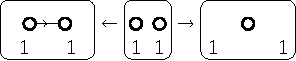
\includegraphics{InclGrphx--2cell--wire_is_identity}
}
\end{equation}
The last is added to 
ensure that the wire 1-cell 
behaves as the identity, 
a property we lose when 
using graphs.
All of these 2-cells, 
we call \emph{basic}.  

It is important to emphasize 
that the basic 2-cells are 
representatives of an equivalence class. 
That is, we have made a decision 
to present these 2-cells 
as a span of cospans 
whose apex is the 
edgeless graph whose 
node set is the disjoint union 
of the inputs and outputs.  
This is certainly not 
the only representative 
we could have chosen,
though it does seem to be 
the most natural choice. 

Forget for a moment that 
our 2-cells are classes and 
think of only the representatives.  
When we compose 
a span of cospans with its dagger, 
we get a non-trivial way to 
rewrite a 1-cell into itself.  
This ought to be 
distinct from the identity rewrite, 
which does nothing.  
However, our choice of 
equivalence classes 
render these the same.
This hints that a higher rewriting structure 
is hiding in the background.  
Indeed, conveying rewrite rules 
as spans of cospans has the 
advantage of including 
higher level rewrite rules in 
by iterating the process of taking spans. 
Currently, we content ourselves
to work within bicategories and 
leave an exploration for
higher structure for another time. 

We now define 
the bicategory which 
categorifies the zx-calculus.

\begin{figure}[h]
	\fbox{%
		\begin{minipage}{\textwidth}
			\centering
			%%%%%%%%%%%%%%%%%%%%%%
			\subcaptionbox{Spider}[\textwidth]{%
				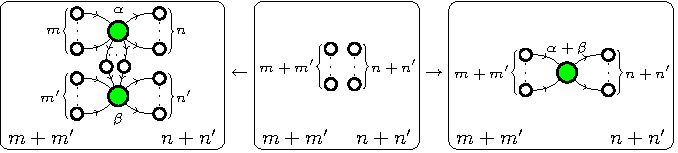
\includegraphics[scale=0.75]{InclGrphx--2cell--spider}
			}
			\linebreak
			\subcaptionbox{Bialgebra}[\textwidth]{%
				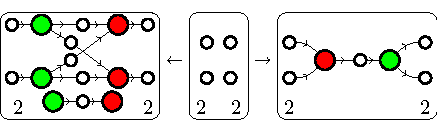
\includegraphics[scale=0.75]{InclGrphx--2cell--bialgebra}
			}
			\linebreak
			\subcaptionbox{Cup}[0.45\textwidth]{%
				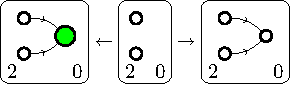
\includegraphics[scale=0.75]{InclGrphx--2cell--cup}
			}
			\subcaptionbox{Copy}[0.45\textwidth]{%
				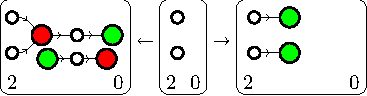
\includegraphics[scale=0.75]{InclGrphx--2cell--copy}
			}
			\linebreak
			\subcaptionbox{Trivial spider}[0.45\textwidth]{%
				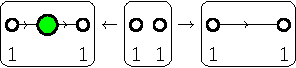
\includegraphics[scale=0.75]{InclGrphx--2cell--trivial_spider}
			}
			\subcaptionbox{$\pi$-copy}[0.45\textwidth]{%
				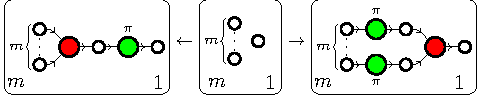
\includegraphics[scale=0.75]{InclGrphx--2cell--pi_copy}
			}
			\linebreak
			\subcaptionbox{$\pi$-commutation}[\textwidth]{%
				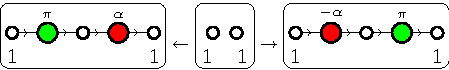
\includegraphics[scale=0.75]{InclGrphx--2cell--pi_commutation}
			}
			\linebreak
			\subcaptionbox{Color change}[\textwidth]{%
				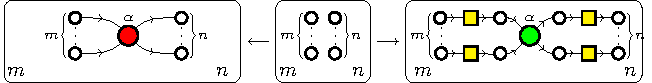
\includegraphics[scale=0.75]{InclGrphx--2cell--color_change}
			}
			\linebreak
			\subcaptionbox{Loop}[0.45\textwidth]{%
				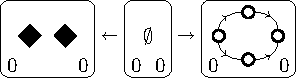
\includegraphics[scale=0.75]{InclGrphx--2cell--loop}
			}
			\subcaptionbox{Diamond}[0.45\textwidth]{%
				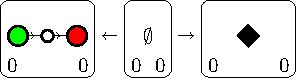
\includegraphics[scale=0.75]{InclGrphx--2cell--diamond}
			}
			%%%%%%%%%%%%%%%%%%%%%%
		\end{minipage}
	}
	\caption{Generating $2$-cells for the bicategory $\underline{\mathbf{zx}}$}
	\label{fig:ZX 2cells generators}
\end{figure}

\begin{defn}
	\label{def:zx bicat}
	Define $\underline{\mathbf{zx}}$ to be 
	the symmetric monoidal and 
	compact closed sub-bicategory 
	of $\mathbf{zxRewrite}$ generated by 
	the basic $1$-cells and basic $2$-cells.
\end{defn}

Working within $\cat{zxRewrite}$
allows us to generate 
$\underline{\mathbf{zx}}$
as an SMCC in this way.
Without having this ambient space,
we cannot be sure that we 
obtain an SMCC bicategory simply
by giving a presentation.

Because $\underline{\mathbf{zx}}$ is 
symmetric monoidal and compact closed, 
it contains twist, 
evaluation, and coevaluation 1-cells 
\begin{equation}
\label{diag:TwistCompact 1cells}
\raisebox{-0.8\height}{
	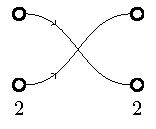
\includegraphics[scale=0.75]{InclGrphx--1cell--zx_braiding}
	\quad \quad \quad
	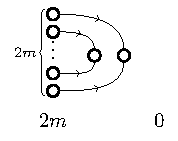
\includegraphics[scale=0.75]{InclGrphx--1cell--zx_evaluation}
	\quad \quad \quad
	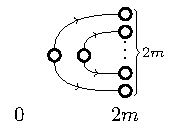
\includegraphics[scale=0.75]{InclGrphx--1cell--zx_coevaluation}
}
\end{equation}
witnessing symmetry and 
the compact structure on $m$.

Horizontal and vertical composition 
are the same as in
	\eqref{eq:Hor and Vert Composition}. 
For example, 
we can compose spider diagrams 
with the same number 
of inputs and outputs:
\[
	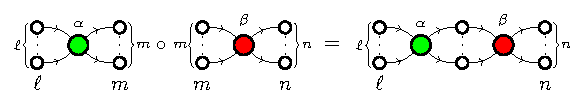
\includegraphics{InclGrphx--example--composing_spiders}
\]
We tensor 1-cells by 
disjoint union, such as
\[
	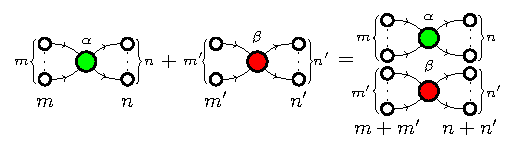
\includegraphics{InclGrphx--equation--tensor_spiders}
\]
With $\underline{\mathbf{zx}}$ defined, 
we turn our focus towards 
presenting the main theorem. 
We start by giving a category that 
is a \emph{decategorification} 
or \emph{truncation} of $\underline{\mathbf{zx}}$.  

\begin{defn}
	\label{def:decat zx}
	Define $|| \underline{\mathbf{zx}} ||$ 
	to be the category whose 
	objects are the 0-cells of $\underline{\mathbf{zx}}$ and 
	whose arrows are the 1-cells of $\underline{\mathbf{zx}}$ 
	modulo the equivalence relation $\sim$ 
	given by: 
	$f \sim g$ if and only if 
	there is a 2-cell $f \Rightarrow g$ 
	in $\underline{\mathbf{zx}}$.
\end{defn}

To be clear, $\sim$ 
is an equivalence relation 
and doesn't merely generate one.  
This follows from 
the symmetry of spans 
and vertical composition.   

\begin{thm}
	\label{thm:decat zx is dagger compact}
	The category $|| \underline{\mathbf{zx}} ||$ 
	is dagger compact via 
	the identity-on-objects functor $\dagger$
	given by 
	\[
	\begin{minipage}{0.4\textwidth}
		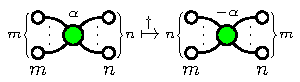
\includegraphics{InclGrphx--functor--dagger_decat_zx_spider_green}
	\end{minipage}
	\begin{minipage}{0.075\textwidth}
		\text{ and } 
	\end{minipage}
	\begin{minipage}{0.4\textwidth}
		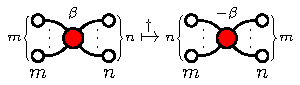
\includegraphics{InclGrphx--functor--dagger_decat_zx_spider_red}
	\end{minipage}
	\]
	as well as by 
	identity on the wire, 
	Hadamard, and diamond morphisms.
\end{thm}
\begin{proof}
	Compact closedness 
	follows from the self duality of objects 
	via the evaluation and coevaluation 
	maps from \eqref{diag:TwistCompact 1cells}. 
	The snake equation is derived by
	\[
	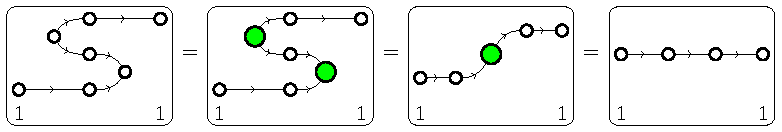
\includegraphics[scale=0.75]{InclGrphx--equation--decat_zx_snake}
	\]
	where the equalities 
	follow from the evident 
	2-cells in $\underline{\mathbf{zx}}$. 
	The extra relation 
		\eqref{eq:2cell wire is identity} 
	ensures that the 
	string of wires is the identity.  
	Showing that $\dagger$
	is a dagger functor is a matter of 
	checking some easily verified details. 
\end{proof}

\begin{thm}
	\label{thm:equiv of zx cats}
	The identity on objects, 
	dagger compact functor 
		$E \colon \mathbf{zx} \to || \underline{\mathbf{zx}} ||$ 
	given by
	\[
	\begin{minipage}{0.175\textwidth}
		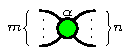
\includegraphics{InclGrphx--generater--green_spider}
	\end{minipage}
		\mapsto
	\begin{minipage}{0.2\textwidth}
		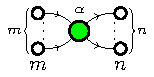
\includegraphics{InclGrphx--1cell--zx_green_spider}
	\end{minipage}
	\quad \quad \quad 
	\begin{minipage}{0.175\textwidth}
		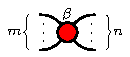
\includegraphics{InclGrphx--generater--red_spider}
	\end{minipage}
	\mapsto
	\begin{minipage}{0.2\textwidth}
		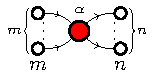
\includegraphics{InclGrphx--1cell--zx_red_spider}
	\end{minipage}
	\]
	\[
	\begin{minipage}{0.1\textwidth}
		
\includegraphics{InclGrphx--generater--wire}
	\end{minipage}
	\mapsto
	\begin{minipage}{0.15\textwidth}
		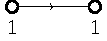
\includegraphics{InclGrphx--1cell--zx_wire}
	\end{minipage}
	\quad \quad \quad 
	\begin{minipage}{0.04\textwidth}
		
\includegraphics{InclGrphx--generater--diamond}
	\end{minipage}
	\mapsto
	\begin{minipage}{0.06\textwidth}
		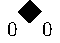
\includegraphics{InclGrphx--1cell--zx_diamond}
	\end{minipage}
	\quad \quad \quad 
	\begin{minipage}{0.1\textwidth}
		
\includegraphics{InclGrphx--generater--hadamard}
	\end{minipage}
	\mapsto
	\begin{minipage}{0.1\textwidth}
		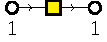
\includegraphics{InclGrphx--1cell--zx_hadamard}
	\end{minipage}
	\]
	is an equivalence of categories.
\end{thm}
\begin{proof}
	That $E$ is identity-on-objects
	implies essential surjectivity.  
	Fullness holds because 
	the generating morphisms for 
	$|| \underline{\mathbf{zx}} ||$  
	are all in the image of $E$. 
	
	Proving faithfulness is more involved. 
	Let $f$ and $g$ be $\mathbf{zx}$-morphisms. 
	Consider representatives
	$\widetilde{Ef}$, $\widetilde{Eg}$
	of $Ef$, $Eg$ obtained by 
	translating directly
	the graphical representation of $f,g$ 
	to open graphs over $S_{\text{zx}}$ 
	as in Examples \ref{ex:graph over Szx}  
	and \ref{ex:open graph over Szx}. 
	It suffices to show that the 
	existence of a 2-cell 
		$\widetilde{Ef} \Rightarrow \widetilde{Eg}$ 
	in $\underline{\mathbf{zx}}$ 
	implies that $f=g$.  
	
	Observe that any 
	2-cell $\alpha$ in 
	$\underline{\mathbf{zx}}$ 
	can be written, 
	not necessarily uniquely, 
	as a sequence 
		$\alpha_1 \square \dotsm \square \alpha_n$ 
	where each $\alpha_i$ is a basic 2-cell, 
	each box is filled with 
	`$\circ_\text{h}$', `$\circ_\text{v}$', or `$+$', 
	and parentheses are right justified.  
	By `$\circ_\text{h}$' and `$\circ_\text{v}$', 
	we mean horizontal and vertical composition. 
	We induct on sequence length.  
	If $\alpha \colon \widetilde{Ef} \Rightarrow \widetilde{Eg}$ 
	is a basic 2-cell, 
	then there is clearly 
	a corresponding basic relation 
	equating $f$ and $g$.  
	Suppose we have a sequence 
	of length $n+1$ such that 
	the left-most square is a `$+$'. 
	Then we have a 2-cell 
	$\alpha_1 + \alpha_2 \colon Ef \Rightarrow Eg$ 
	where $\alpha_1$ is a basic 2-cell 
	and $\alpha_2$ can be 
	written with length $n$.   
	By fullness, we can write 
	$\alpha_1 + \alpha_2 \colon Ef_1 + EF_2 \Rightarrow Eg_1 + Eg_2$ 
	where $\alpha_i \colon Ef_i \Rightarrow Eg_i$.   
	This gives that $f_i = g_i$  
	and the result follows.  
	A similar argument handles 
	the cases when the 
	left-most operation is 
	vertical or horizontal composition.
\end{proof}
 
%%%%%%%%%%%%%%%%%%
%%%%%%%%%%%%%%%%%%
% 
\end{document}
%
%%%%%%%%%%%%%%%%%%
%%%%%%%%%%%%%%%%%%
